\documentclass[12 pt]{article}
\usepackage[all]{xy}
%\documentclass[13pt]{article}
\usepackage{amssymb}
%\usepackage{verbatim}
\usepackage{amsmath}
\usepackage{setspace}
\usepackage{graphicx}
\usepackage{graphics,graphicx}
\usepackage[demo]{graphicx}
\usepackage{subfig}
\usepackage{pgf,color}
\usepackage{epstopdf}
\usepackage{epsfig,textpos,mathrsfs}
\usepackage{amsthm}
\newtheorem{definition}{Definition}[section]
\usepackage[utf8]{inputenc}
\usepackage[english]{babel}
\usepackage{amsthm}
\usepackage{layout}
%%%%%%%%%%%%%%%%%%%%%%%%%%%%%%%%%%%%%%%%%%%%%%%
\setlength{\textwidth}{6.5in}
\setlength{\textheight}{8.5in}
\setlength{\oddsidemargin}{0pt}
\setlength{\evensidemargin}{0pt}
\setlength{\topmargin}{0pt}
%%%%%%%%%%%%%%%%%%%%%%%%%%%%%%%%%%%%%%%%%%%%%%%
\newtheorem{remark}{Remark}[section]
\newtheorem{theorem}{Theorem}[section]
\newtheorem{lemma}{Lemma}[section]
\newtheorem{proposition}{Proposition}[section]
\newtheorem{corollary}{Corollary}[section]
\newtheorem{example}{Example}[section]
\theoremstyle{definition}
\theoremstyle{remark}
\newcommand{\R}{\mathbb{R}}
\newcommand{\N}{\mathbb{N}}
\newcommand{\h}{\mathcal{H}}
\newcommand{\Z}{\mathbb{Z}}
\newcommand{\B}{\mathcal{B}}
\newcommand{\A}{\mathcal{A}}
\newcommand{\Y}{\mathcal{Y}}
\newcommand{\X}{\mathcal{X}}
\newcommand{\G}{\mathcal{G}}
\newcommand{\T}{\mathbb{T}}
\newcommand\norm[1]{\left\lVert#1\right\rVert}

\usepackage{afterpage}

\newcommand\blankpage{%
    \null
    \thispagestyle{empty}%
    \addtocounter{page}{-1}%
    \newpage}


\linespread{1.1}


\begin{document}

\begin{center}
\begin{LARGE}
\textbf {Calculus On Normed Vector Spaces}
\end{LARGE}
\begin{center}
\end{center}
{\begin{Large}
\textbf{MTP REPORT} \\
\end{Large}}
\today
%(For enhancement of JRF to SRF)
\end{center}

\vspace{45mm}
\begin{center}
Submitted by


\textbf{Joydeep Medhi}

\bf Entry No. 2013MT60599
\vspace{15mm}

\textit{Supervisor}

\textbf{Prof. Amit Priyadarshi}

\end{center}
\vspace{2cm}
\begin{center}

\includegraphics[height=3.5cm]{iitlogo.jpg}
\end{center}
\begin{center}
\textbf{{Department of Mathematics\\
Indian Institute of Technology Delhi,\\
New Delhi, INDIA}}
\end{center}
\thispagestyle{empty}
\thispagestyle{empty}

%\afterpage{\blankpage}


\section{Introduction}

The aim of the project is to study the notion of derivatives on general normed vector spaces and do Calculus on them. We will also look at some applications of these concepts.
Till \textbf{section 5} was done for Mid-Term presentation and from \textbf{section 6 to section 10} is done after Mid-Term Presentations.

\textbf{Norm}:
We will suppose that all vector spaces are real. Let $E$ be a vector space. A mapping $ \norm{.}: E\rightarrow \mathbb{R} $, is said to be a \textit{norm} if, for all $\textit{x, y} \in E$ and $\lambda \in \mathbb{R}$ 
\\
\hspace*{2cm} $\norm{x}\geq 0$\\
\hspace*{2cm} $\norm{x} = 0 \Leftrightarrow x = 0$\\
\hspace*{2cm} $\norm{\lambda x} = |\lambda|\norm{x}$\\ 
\hspace*{2cm} $\norm{x + y} \leq \norm{x} + \norm{y}$
 
The pair $(E, \norm{.})$ is called a \textit{normed vector space} and we say that $\norm{x}$ is the norm
of $x$.\\
%%%%%%%%%%%%%%%%%%%%%%%%%%%%%%%%%

\textbf{Continuity}: Suppose now that we have two normed vector spaces, $(E, \norm{.}_{E})$ and $(F, \norm{.}_{F})$. Let A be a subset of E, $ f $ a mapping of $A$ into $F$ and $a \in A$. We say that $f$ is \textit{continuous} at $a$ if the following condition is satisfied: \par
for all $\epsilon > 0$, there exists $\delta > 0$ such that, if $x \in A$ and $\norm{x-a}_{E} < \delta$,\\ then $\norm{f(x) - f(a)}_{F} < \epsilon$ \\
If $f$ is \textit{continuous} at every point $a \in A$, then we say that $f$ is \textit{continuous} on $A$.\\

\proposition{The norm on a normed vector space is a continuous function}.
\normalfont
\proof We have 
$\norm{x} = \norm{x-y+y} \leq \norm{x-y} + \norm{x} \Rightarrow \norm{x} - \norm{y} \leq \norm{x-y}$\\
In similar way,  $\norm{y} - \norm{x} \leq \norm{y-x}.$ As $\norm{y-x} = \norm{x-y}$, We get
\begin{center}
$|\norm{x}-\norm{y}| \leq \norm{x-y}$
\end{center} 
And hence the continuity.\\
%%%%%%%%%%%%%%%%%%%%%%%%%%%%%%%%%%%%%%

\proposition {Let E and F be normed vector spaces, $A \subseteq E, a \in A$, f and g are mappings from E into F and $\lambda \in \mathbb{R}$ .
\normalfont

\item[\hspace{1cm} $\bullet$]If $f$ and $g$ are continuous at a, then so is $f + g$.
\item[\hspace{1cm} $\bullet$]If $f$ is continuous at a, then so is $\lambda f$.
\item[\hspace{1cm}  $\bullet$]If $\alpha$ is a real-valued function defined on $E$ and both $f$ and $\alpha$ are continuous at a, then so is $\alpha f$.}

\newpage
%%%Section 
\section{Differentiation}
\normalfont
In this section we will be primarily concerned with extending the derivative defined
for real-valued functions defined on an interval of $\R$. We will also consider minima
and maxima of real-valued functions defined on a normed vector space.

\subsection{Directional Derivatives}

Let $O$ be an open subset of a normed vector space $E$, $f$ a real-valued function
defined on $O$, $a \in O$ and u a nonzero element of $E$. The function $f_{u}:t\rightarrow f(a +tu)$ is defined on an open interval containing 0. If the derivative $\frac{df_{u}}{dt}(0)$ is defined, i.e., if the limit
\begin{center}
$\lim_{t\to 0} \dfrac{f(a+tu)-f(a)}{t}$
\end{center}
exists, then it is called the \textit{directional derivative} of $f$ at $a$ in the direction of $u$, i.e. $\partial_{u}f(a)$ . \\

If $E = \R_{n}$ and $e_{i}$ is its standard basis, then the directional derivative $\paerial{e_{i}}f(a)$ is called the $i$ th partial derivative of $f$ at a, or the derivative of $f$ with respect to $x_{i}$ at $a$.

\begin{center}
$\dfrac{\partial f}{\partial{x_{i}}} = \lim_{t \to 0} \dfrac{f(a_{1},..,a_{i} + t,...,a_{n}) - f(a_{1},....,a_{n})}{t}$
\end{center}

If for every point $x \in O$, the partial derivative $\dfrac{\partial f}{\partial x_{i}} (x) $ is defined, then we obtain the function i th partial derivative defined on $O$. If these functions are defined and continuous for all i , then we say that the function $f$ is of class $ C^{1} $.


Suppose now that $O$ is an open subset of $\R^n$ and $f$ a mapping defined on $O$ with image in $\R^m$. $f$ has m coordinate mappings $f_1,...., f_m$. If $a \in O$ and the partial derivatives $\dfrac{\partial f_i}{\partial x_j} $ of $a$, for $1 \leq i \leq m$ and $1 \leq j \leq n$, are all defined, then the $m \times n $ matrix

\begin{center}
\[
J_f (a)=
  \begin{bmatrix}
    \dfrac{\partial f_1}{\partial x_1} & . ~ . ~ . & \dfrac{\partial f_1}{\partial x_n}  \\
    . & . & . \\
    . & . & . \\
    . & . & . \\
    \dfrac{\partial f_m}{\partial x_1} & . ~ . ~ . & \dfrac{\partial f_m}{\partial x_n} 
  \end{bmatrix}
\]
\end{center}

is called the \textit{Jacobian Matrix} of $f$ at $a$.\\

\newpage

\subsection{The Differential}

Let $E$ and $F$ be normed vector spaces, $O$ an open subset of $E$ containing 0, and $g$ a mapping from $O$ into $F$ such that $g(0) =  0$. If there exists a mapping \epsilon, defined on a neighbourhood of $0 \in E$ and with image in $F$ , such that $\lim_{h \to 0} \epsilon(h) = 0$ and \\~\\
\hspace*{2cm} $g(h) = \norm{h}_E \epsilon(h)$,\\~\\
then we write $g(h) = o(h)$ and say that $g$ is \textit{"small o of h"}. \\

The condition $g(h) = o(h)$ is independent of the norms we choose for two spaces $E$ and $F$. \\
\par 
Let $O$ be an open subset of a normed vector space $E$ and $f$ a mapping from $O$
into a normed vector space $F$ . If $a \in O$ and there is a continuous linear mapping $\phi : E \rightarrow F$ such that \\~\\
\hspace*{1cm} $ f(a+h) = f(a) + \phi (h) + o(h) $ \\

when $h$ is close to 0, then we say that $f$ is \textit{differentiable} at $a$.\\



\proposition{Let f be a mapping defined on an open subset O of a normed
vector space E with image in the cartesian product $F =F_1 \times . . . \times F_p$. Then $f$ is
differentiable at $a \in O$ if and only if the coordinate mappings $f_i$ , for $i = 1,...,p $ ,
are differentiable at a.\\
\hspace*{3cm} $ f'(a) = (f_1 '(a),....., f_p '(a)) $}

\normalfont \\~\\

Suppose that dim $E$ = $n < \infty$ and that $e_i$ is a basis of $E$. If $ x = \sum_{i=1}^{n} x_i e_i$, then\\
\begin{center}
$ f'(a)x = \sum_{i=1}^{n} x_i f'(a) e_i = \sum_{i=1}^{n} \partial_{e_i} f(a) e_i^*(x)$,
\end{center}

where $(e_i^*)$ is the dual basis of $(e_i)$. We thus obtain the expression. If $E = \R^n$ and $(e_i)$ is its standard basis, then we usually write $dx_i$ for $e_i^*$. This gives us the expression \\
\begin{center}
$ f'(a)x = \sum_{i=1}^{n} \dfrac{\partial f}{\partial x_i} (a) dx_i $.
\end{center}

\textbf{Differentiability at a given point}:
If we wish to determine whether a real-valued function $f$ defined on an open subset of $\R^n$ is differentiable at a given point $a$, then first we determine whether all its partial derivatives at $a$
exist. If this is not the case, then f is not differentiable at a.\\ 
If all the partial derivatives exist, then we know that the only possibility for $f'(a)$ is the linear function $ \phi = \sum_{i=1}^{n} frac{\partial f}{\partial x_i} (a) dx_i $. We consider the expression,\\

\begin{center}

$ \dfrac{f(a+h) - f(a) - \phi (h)}{\norm{h}} = \epsilon (h)$
\end{center}

If $\lim_{h \to 0} \epsilon (h) =  0$, then $f$ is differentiable at a, otherwise it is not. \\

\subsection{Differentials of Compositions}

Let $E$, $F$ and $G$ be normed vector spaces, $O$ an open subset of $E$, $U$ an open subset of $F$ and $f : O \rightarrow F$ , $g : U \rightarrow G$ be such that $f(O) \subset U$ . Then the mapping $g \circ f$ is defined on $O$.

\theorem{If f is differentiable at a and g is differentiable at f(a), then $g \circ f$ is differentiable at a and\\
\hspace*{4cm} $  (g \circ f)' (a) = g'(f(a))\circ f'(a) $.\\
This expression is referred to as Chain Rule.}
\\

\corollary{If in the above theorem the normed vector spaces are euclidean
spaces, then \\
\hspace*{4cm} $ J_{g \circ f} (a) = J_g (f(a)) \circ J_f (a)$. }

\normalfont

\subsection{Differentiability of the Norm}
If $E$ is a normed vector space with norm $\norm{.}$, then $\norm{.}$ is itself a mapping from $E$ into $\R$ and we can study its \textit{differentiability}. We will write $Df(\norm{.}) (x)$ for differentiability of the norm at x (if exists).

\proposition {Norm is not differentiable at the origin.}
\proof Suppose $Df(\norm{.})$ exists. Then for small non-zero values of $h$, we have \\
\begin{center}
$ \norm{h} =  Df(\norm{.})(0)h + o(h) \Rightarrow \lim_{h \to 0} \left( 1 - Df(\norm{.}) \dfrac{h}{\norm{h}} \right) = 0 $
\end{center} And
\begin{center}
$ \norm{h} = \norm{-h} =  -Df(\norm{.})(0)h + o(h) \Rightarrow \lim_{h \to 0} \left( 1 + Df(\norm{.}) \dfrac{h}{\norm{h}} \right) = 0$
\end{center}


\newpage

\section{Mean Value Theorem}

\theorem Let f be a real-valued function defined on a closed bounded interval $[a,b] \subset \R$. If f is continuous on $[a,b] $ and differentiable on $(a,b0 $ then there is a point $c \in (a,b)$ such that
\begin{center}
$ f(b) - f(a) = \dot{f}(c)(b-a)$
\end{center}

\subsection{Generalization of Mean Value Theorem}

\theorem Let $O$ be a open subset of a normed vector space $E$ and $a,b \in E$ with $[a,b] \in O$. If $f:O \to \R$ is differentiable , then there is a element $c \in (a,b)$ such that 
\begin{center}
$ f(b) - f(a) = f'(c)(b-a)$
\end{center}

\remark{ If $E = \R^n$ then this result can be written as\\
\hspace*{3cm}	$f(b) - f(a) = \sum_{i=1}^{n} \dfrac{\partial f}{\partial x_i}(c)(b_i - a_i)$}\\


\normalfont

\theorem Let $[a,b]$ be an interval of $\R$, $F$ a normed vector space and $f:[a,b] \to F$ and $g: [a,b] \to \R$ both continuous and differentiable on $(a,b)$. If $\norm{\dot{f}(t)} \leq \dot{g}(t)$ for all $t \in (a,b)$, then \hspace*{3cm} $\norm{f(b) - f(a)}_F \leq g(b) - g(a)$.
		
\vspace*{4mm}

\corollary Let $E$ and $F$ are normed vector spaces, $O$ an open subset of $E$ and $f:O \to F$ differentiable on $O$. If the segment $[a,b] \subset O$ ,then\\
\hspace*{3cm}   $ \norm{f(b)-f(a)}_F  \leq sup_{x \in (a,b)} |f'(x)|_{L(E, F)} \norm{b-a}_E $

\normalfont
\subsection{Partial Differentials}
In this section we will generalize the notion of partial derivatives and its results.

Let $E_1, E_2,....,E_n$ and $F$ be normed vector spaces. We set\\
\hspace{3cm} $E = E_1 \times.......\times E_n$ and define a norm on $E$\\

\hspace*{3cm} $ \norm{(x_1,...,x_n)}_E = $max_k $\norm{x_k}_{E_k}$.\\


Now let $O$ be an open subset of $E$ and $f$ a mapping from $O$ into $F$ . If we take a
point $a \in O$ and let the kth coordinate vary and fix the others, then we obtain a
mapping $f_{a,k}$ from $E_k$ into $F$ , defined on an open subset of $E_k$ containing $a_k$.\\

If $f_{a,k}$ is differentiable at $a_k$, then we call the differential $f'_{a,k}(a_k) \in L(E_k, F)$
the \textit{kth partial differential of f at a} and write it as $\partial_k f(a)$ for $f'_{a,k}(a_k)$. 

\section{Higher Derivatives and Differentials}

Let $O \subset \R^n$ be open and $f$ a real valued function defined on $O$. If the function $\frac{\partial f}{\partial x_i}$ is defined on $O$, then we can consider the existance of its partial derivatives. If $ \frac{\partial}{\partial x_i}(\frac{\partial f}{\partial x_i})(a)$ exists, then we write for this derivative $\frac{\partial^2 x}{\partial x_j \partial x_i}(a)$ if $i \neq j$ and $\frac{\partial^2 x}{\partial^2 x_i}(a)$ if $i = j$.

If these functions are defined and continuous for all pairs $(j,i)$, then we say that $f$ is of class $C^2$.

We say that continuous functions are of class $C^0$ . If a function is of class $C^K$ for all
$K \in \N$, then we say that $f$ is of class $C^{\infty}$ , or smooth.

\subsection{Schwarz’s Theorem}
\theorem Let $O \subset \R^2$ be open and $f: O \to \R$ be such that the second partial derivatives $\frac{\partial^2 f}{\partial x \partial y}$ and $\frac{\partial^2 f}{\partial y \partial x}$ are defined on $O$. If these functions are continuous at $(a,b) \in O$, then \\
\hspace*{3cm} $\dfrac{\partial^2 f}{\partial x \partial y}(a,b)= \dfrac{\partial^2 f}{\partial y \partial x}(a,b)$.

\subsection{Multilinear Mapping}
\normalfont

Second and higher differentials are more difficult to define than second and higher
derivatives. The natural way of defining a second differential would be to take the
differential of the mapping $x \mapsto f'(x)$. Unfortunately, if $E$ and $F$ are normed
vector spaces and $f$ a differentiable mapping from an open subset of $E$ into $F$ ,
then the image of $f'$ lies not in $F$ but in $L(E,F)$. This means that the differential
of $f'$ lies in $L(E,L(E,F))$.\\

\subsection{Higher Differentials}
Let $E$ and $F$ be normed vector spaces and $O$ an open subset of $E$. If $f: O \to F$ is differentiable on an open neighbourhood $V$ of $a \in O$, then the mapping\\
\hspace*{3cm} $f': V \mapsto L(E,F), x \mapsto f'(x)$ is defined.\\


As we said in the previous section, if $f'$ is differentiable at $a$, then we would be tempted to define the second differential $f^{(2)}(a)$ of $f$ at $a$ as $f''(a) = (f')'(a)$. However, in this way $f^{(2)}(a) \in L_2(E,F)$ and it is difficult to work with these higher order spaces. Hence we proceed in a different way.\\

We will define linear continuous mappings $\Phi_k$ from $L_k (E, F) \to L(E^k, F)$. \\

we define k-differentiability and the kth differential $f^{(k)}(a)$ for higher values of k. We will sometimes write $f^{(1)}$ for $f'$. To distinguish the differential in $L_k(E; F)$  corresponding to $f^{(k)}(a)$, we will write $f^{[k]}$ for it, i.e., $\Phi_k (f^{[k]}(a)) = f^{(k)}(a)$.\\

\subsection{Taylor Formulas}
\normalfont
Some useful notation

1) Let $E$ and $F$ be normed vector spaces, $O$ an open subset of $E$ containing 0 and $g$
a mapping from $O$ into $F$ such that $g(0) = 0$. If there exists a mapping $\epsilon$, defined
on a neighbourhood of $0 \in E$ and with image in $F$, such that $lim_{h \to 0} \epsilon (h)$ and \\
\hspace*{3cm}			$g(h) = \norm{h}_E^k \epsilon(h)$,\\

then we will write $g(h) = o(\norm{h}_E^k)$ or $g(h) = o(\norm{h}^k)$ when the norm is understood. If k =1, then $o(\norm{h}) = o(h)$\\~\\

2) If $E$ is a normed vector space and $h$ is a vector in $E$, then we will write $h^k$ for
the vector $(h,.......,h) \in E^k$ .\\

\theorem \textbf{(Taytor's formula, asymptotic form)}. Let $E$ and $F$ be normed vector spaces, $O$ an open subset of $E$ and $a \in O$. If $f: O \to F$ is $(k-1)$-differentiable and $f^{(k)}(a)$ exists, then for $x$ is sufficiently small \\
\qquad $ f(a+x) = f(a)  + f^{(1)}(a)(x) + \frac{1}{2} f^{(2)}(a)(x^2) +....+\frac{1}{k!} f^{(k)}(a)(x^k) + o(\norm{h}^k)$.

\subsection{Extrema: Second Order Condition}
\normalfont

A local extremum of a differentiable function is always a critical point. We now suppose that the function is 2-differentiable at the critical point. We will discuss local minima; analogous results for local maxima can be easily obtained by slightly modifying the argument

\proposition Let $O$ be an open subset of a normed vector space $E$, $a \in O$ and $f$ a real-valued function defined on $O$ having a second differential at $a$. If $a$ is a local minimum, then for $h \in E$ \\

\hspace*{4cm} $f^{(2)}(a)(h,h) \geq 0$

\section{Hilbert Space}
\normalfont
A vector space $E$ over the field $F$ together with an inner product, i.e., with a map

\hspace{2cm} $<.,.>$ : $E$ x $E \to F$ \\
which follows the three axioms for all vectors $\in E$ Positive-definiteness, Linearity in first argument, Conjugate symmetry

Then the pair $( E, <,>)$ is called an inner product space, for $x \in E$ , $\norm{x}$ is defined as $ \sqrt{ <x,x>} $.\\

If $E$ is an inner product space and complete with the norm derived from the inner product, Then $E$ is said to be a \textbf{Hilbert Space}.

\subsection{The Riesz Representation Theorem}
If H is a Hilbert space, then by the Riesz representation theorem, we may associate an element of H to a continuous linear form.

Before looking at the general Theorem, let us see what
happens in $\R^n$ . If $l$ is a linear form defined on $\R^n$, $(e_i)$ its standard basis and 
$x$ = $\sum_{i = 1}^{n} x_i e_i$ then

\hspace*{2cm} $l(x) = \sum_{i=1}^{n} x_i l(e_i) = x . w$, where $w = (l(e_1), ...., l(e_n))$.

If $\overline{w}$ is such that $l(x) = x. \overline{w}$ for all $x \in \R^n$, then $x.(w - \overline{w}) = 0$ for all $x \in \R^n$, it follows that $ w - \overline{w} = 0$. Hence, the element $w$ such that $l(x) = x.w$ for all $x$ is \textbf{unique}.

\theorem Let $l$ be a continuous linear form defined on a Hilbert space $H$ . Then there is a unique element $a \in  H$ such that

\hspace*{3cm} $l(x) = <x, a>$ \\
for all $x \in H$. In addition, $|l|_{H^{*}} = \norm{a}$.

\normalfont
\subsection{Convex Functions}
Let $X$ be a convex subset of a vector space $V$ . We say that $f$ : $X \to \R$ is \textbf{convex} if for all $x, y \in X$ and $ \lambda \in (0,1)$ we have 

\hspace*{2cm} $ f\left( \lambda x + (1- \lambda ) y\right) \leq \lambda f(x) + (1-\lambda) f(y)$

If this inequality is strict when $x \neq y$, then we say that $f$ is \textbf{strictly convex}.

\subsection{Convex Hull}
Let $E$ be a vector space and $x_1 ,..., x_n \in E$. We say that $y \in E$ is a \textit{convex combination} of the points $x_1 ,..., x_n$ if there exists $\lambda_1 ,..., \lambda_n \in [0,1]$ with $\sum_{i=1}^n \lambda_i = 1$ such that $ y = \sum_{i=1}^n \lambda_i x_i$.

If $X$ is a nonempty subset of $E$, then we
define \textit{co X} , the convex hull of $X$ , to be the set of points $y \in E$ which are convex combinations of points in $X$.

\textbf{Definition.} A subset $X$ of a vector space $E$ is convex if and only if \textbf{co} $X = X$.

\subsection{Continuity of Convex functions}
\lemma If P is a bounded nonempty polyhedron in a finite-dimensional normed vector space E and f is a convex function defined on E, then f has an upper bound on P.

\theorem Let $X$ be a finite dimensional normed vector space $E$ and $f: X \to \R$ is convex. If $x \in int X$, then $f$ is continuous at $x$.

\corollary If a convex function is defined on an open subset of a finite-dimensional normed vector space, then it is continuous.
\normalfont
\subsection{Differentiable Convex Functions}
Let O be an open subset of a normed vector space $E$ and $f$ a real-valued differentiable functions defined on $O$. If $X \subset O$ is convex and $x, y \in X$, then the following are equivalent:
\begin{itemize}
\item $f$ is convex on X.
\item $f(y) - f(x) \geq f'(x)(y-x)$
\item $ (f'(y) - f'(x))(y-x) \geq 0$
\end{itemize}

\remark From third condition we deduce that, if $f$ is differentiable on
an open interval $I$ of $\R$, then $f$ is convex (resp. strictly convex) if and only if the
derivative of $f$ is increasing (resp. strictly increasing) on $I$.
\normalfont

\section{The Inverse Mapping Theorem}
\proposition Let $E$ and $F$ be Banach spaces, $O \subset E$ and $U \subset F$ open
sets and $f : O \to U$ a differentiable homeomorphism. If $a \in O$ and $f'(a)$ is invertible then $f^{-1}$ is differentiable at $b = f(a)$.

In addition, if $f$ is of class $C^1$ then there is a open neighbourhood $O'$ such that $f_{|O'}$ is a $C^1$-diffeomorphism onto its image.

\theorem Let $E$ and $F$ be Banach spaces, $O \subset E$ and $f : O \to F$ of class $C^1$. If $a \in O$ and $f'(a)$ is invertible, then there is an open neighbourhood $O'$ of such that $f_{ |O'}$ is a $C^1$-diffeomorphism onto its image.

\remark Under the conditions of the theorem, 
\begin{itemize}
\item $f_{ |O'}$ is a $C^1$-diffeomorphism onto its image. In fact if $f$ is of class $C^k$, then $f_{ |O'}$ is a $C^k$-diffeomorphism.

\item If a mapping $f$ is such that each point in its domain has an open neighbourhood
$O$ such that $f$ restricted to $O$ defines a diffeomorphism onto its image, then we
say that $f$ is a \textbf{local diffeomorphism}.
\end{itemize}
%%%%%%%%%%%%%%%%%%%%%%%%%%%%%%%%%%%%%%%%%%%%%%%%%%%%%%
%%%%%%%%%%%%%%% New Work%%%%%%%%%%%%%%%%%%%%%%%%%%%%%%%
\normalfont
\section{Vector Fields}
Let E be a normed vector space and O an open subset of E. A continuous mapping $X$ from $O$ into $E$ is called a vector field. If $X$ is of class $C^k$ , with $k \geq 1$, then
we refer to $X$ as a vector field of class $C^k$ . If $I$ is an open interval of $\R$ and $\phi$ a differentiable mapping from $I$ into $O$ such that\\
\hspace*{5cm} $\dot{\phi}(t) = X(\phi (t))$\\

for all $t \in  I$ , then we say that $\phi$ is an integral curve of $X$ or a solution of the first-order differential equation $\dot{x}= X(x)$. As $X$ and $\phi$ are both continuous, so is $X \circ \phi$
and it follows that $\phi$ is of class $C^1$.

An integral curve $\phi$ defined on an open interval $I$ is a maximal integral curve if it cannot be extended to an integral curve defined
on an open interval strictly containing $I$ .

\textbf{Notation.} Let $a \in R$. We will write $T$ a for the translation mapping of $R$ into $R$ defined by\\
\hspace*{4cm} $T_a(t) =  t-a$

The integral curves of a vector field have an important elementary property, namely they are invariant under translation.

\proposition{Let $\phi : I \to O$ be an integral curve of a vector field $X :O \to E$ and $a \in \R$. Then $\phi \circ T_a$ a is an integral curve of $X$ defined on $I + a$.
In addition, $\phi \circ T$ a is maximal if and only if $\phi$ is maximal.}\\

\normalfont
There is a slight variety of vector fields which is time-dependent vector fields. Suppose that $E$ and $O$ are as above, $J$ an open interval of $\R$ and $Y$ a continuous mapping from $J \times O \to E$. Then we say that $Y$ is a \textbf{time-dependent vector field}. In this case, for each $t \in J$ , the mapping $Y_t : x \mapsto Y (t, x)$ is a \textbf{vector field}.

An integral curve of Y is a differentiable mapping $\phi$ from an open interval $I \subset J$ into $O$ such that\\
\hspace*{4cm} $\dot{\phi}(t) = Y(t, \phi (t))$\\

for $t \in I$. As $Y(t,\phi(t))$ is continuous, $\phi$ is of class $C^1$.

\subsection{Existence of Integral Curves}
Let $X : O \to E$ be a locally Lipschitz vector field and $x_0 \in O$. There exists
a closed ball $\Bar{B}( x_0, r)$, with $r > 0$, and a constant $K > 0$ such that $X$ is restricted to  $\Bar{B}( x_0, r)$ is K-Lipschitz. As $X$ is Lipschitz on $\Bar{B}( x_0, r)$,$X$ is bounded on $\Bar{B}( x_0, r)$. We take the norm,\\

\hspace*{4cm} $M = \sup_{x \in \Bar{B}( x_0, r)$} \norm{X(x)}$.\\

\theorem If $E$ is a Banach space, $t_0 \in \R$ and $\epsilon > 0$, with $M < r$, then there is a unique integral curve $\phi$ defined on the interval $I_\epsilon = (t_0 - \epsilon, t_0 + \epsilon)$ satisfying the condition $\phi (t_0) = x_0$. The image of $\phi$ lies in the open ball $B(x_0, r)$.

\proposition Let $\phi$ and $\psi$ be integral curves of the vector field $X$ defined on the same open interval $I$. If $t_0 \in I$ and $\phi (t_0) = \psi (t_0)$, then $\phi (t) = \psi(t) $ for all $t \in I$.

\theorem Let $t_0 \in \R$ and $x_0 \in O$, the domain of the vector field $X$. Then there is a unique maximal integral curve $\phi$ with $\phi (t_0) = x_0$.

\proof From \textit{Theorem 7.1} there exists an interval $\Tilde{I}$ on which an integral curve $\Tilde{\phi}$ is defined with $\Tilde{\operatornamewithlimits{} (t_0) = x_0$.

Let $I$ be the union of all such open intervals. For $t \in I$ we take any one of these integral curves $\Tilde{\phi}$ defined at $t$ and set $\phi (t) = \Tilde{\phi} (t)$. From the preceding proposition $\phi (t)$ does not depend on the integral curve  Q which we have chosen, so $\phi$ is well-defined. Clearly $\phi$ is maximal and $\phi (t_0) = x_0$. 

If $\psi : I_1 \to O$ is another maximal integral curve and $\psi (t_0) = x_0$ ,then $I_1 \subset I$ and, because $\psi$ is maximal, $I_1 = I$. Using \textit{Proposition 7.2} we see that $\psi = \phi$. Hence Proved. \qedsymbol \\


Now consider a class of vector fields which is particularly easy to study. Let
$E$ be a Banach space and $A \in L(E)$. If we set $X(x) = Ax$ for $x \in E$, then $X$ is a smooth vector field defined on $E$. Such vector fields are called \textbf{linear vector fields}.

\hspace*{4cm} $\norm{A(x) - A(y) }= |A| \norm{x - y}$\\

$X$ is Lipschitz. Let us consider the mapping $\alpha : \R \to L(E)$, $t \mapsto \exp{(tA)}$.

\proposition $\dot{\alpha} (t) = \exp{(tA)} \circ A = A \circ \dot{\alpha} (t) = \exp{(tA)}$\\

\normalfont
Now let us take $x_0 \in E$ and consider the mapping $\phi : \R \to E$, $t \mapsto \exp{(tA)}x_0$

\theorem{$\phi$ is the maximal integral curve of the linear vector field $X(x) = Ax$ with $\phi (0) = x_0$.}

\normalfont
\textbf{Remark.} If $t_1 \neq 0$ and we require the maximal integral curve with $\psi (t_1) = x_0$,
then it is sufficient to set $\psi =  \phi \circ T_{t_1}$ .

We will often write $\Phi (t, t_0, x_0)$ for the maximal integral curve $\phi$ satisfying the condition $\phi (t_0) = x_0)$ and $I_{t_0 ,x_0}$ for the domain of $\phi$. If $O$ is the domain of the vector field and we set

$D = \cup_{t_0 \in \R, x_0 \in O} I_{t_0, x_0} \times {t_0} \times {x_0} $,\\
then $\Phi$ defines a mapping from $D$ into $O$. We will refer to $\Phi$ as the \textbf{flow of the vector field} $X$.\\

\textbf{Example.} Let
$E$ be a Banach space and $A \in L(E)$. If we set $X(x) = Ax$ for $x \in E$, then $X$ is a smooth vector field defined on $E$.\\

Then, $D = \R \times \R \times E$ and $\Phi (t, t_0, x_0) = \exp{((t-t_0)A)} x_0$. $\Phi$ is continuous on $D$.

\subsection{Initial Conditions}
If $x_0$ is in domain of a vector field and $t_0 \in \R$, then there is a unique maximal integral curve $\phi$ with $\phi (t_0) = x_0$. The pair $(t_0, s_0)$ is called the initial condition that satisfy $\phi$.

\lemma \textbf{Gronwell's Inequality. } Let $f$ and $g$ are continuous functions defined on closed interval $I = [a,b]$ into $\R_+$. If there is a constant $c$ such that for $t \in I$\\

\hspace*{4cm} $f(t) \leq c + \int_a^t f(s)g(s) ds$,\\
then for $t \in I$, we have\\
\hspace*{4cm} $f(t) \leq c \exp{\int_a^t g(s)ds}$.

\corollary Let $f$ is continuous functions defined on closed interval $I = [a,b]$ into $\R_+$. If there is a constant $c \geq 0$ and $k \geq 0$ such that for $t \in I$\\

\hspace*{4cm} $f(t) \leq c + \int_a^t f(s)g(s) ds$,\\
then for $t \in I$, we have\\
\hspace*{4cm} $f(t) \leq ce^{k(t-a)}$.\\

\normalfont
Now we will see how the distance between two vector fields are defined.

\theorem Let $O$ be an open subset of the Banach Space $E$ and $X$ a $K-Lipschitz$ vector field defined on $O$. If $\phi$ and $\psi$  are integral curves defined on the interval $I = [t_0, t_1]$, $\phi (t_0) = x_0$ and $\psi (t_0) = y_0$, then\\
\hspace*{5cm} $\norm{\phi (t) - \psi(t)} \leq \norm{x_0 - y_0} e^{K(t-t_0)}$, for all $t \in I$.
\normalfont
\subsection{Complete Vector Field}
A vector field is said to be complete if all its maximal integral curves are defined on $\R$. from previous theory we can say that, linear vector fields are complete.

Clearly, if a vector field is complete, then the domain of its flow is $\R^2 \times O$, where $O$ is the domain of the vector field.\\

Let $E$ be a normed vector space, $O$ an open subset of $E$ and $X$ a vector field defined on $O$. If $f$ is a real-valued $C^1$ -function defined on $O$ such that, for any integral curve $\phi$ of $X$, $f \circ \phi$ is constant, then we say that $\phi$ is a first integral of $X$. 

If f is a function of constant value, then f is a first integral; though, we will study non constant first integrals.

\proposition Let $E$ be a Banach space, $O$ an open subset of $E$ and $X$ a vector field defined on $O$. A $C^1$ function $f : O \to \R$ is a first integral of $X$ if and only if $f'(x) X(x) = 0$ for all $x \in O$.\\ \normalfont
\textbf{Example. } Consider the vector field $X$ defined on $\R^3$ by

\hspace*{3cm} $X(x,y,z) = (4xy - 1, -2x(1+2z), -2x(1 + 2y))$.\\

If $f : \R^3 \to \R$ is defined by $f(x,y,z) = y + y^2 - z - z^2$, then\\
\hspace*{3cm} $\nabla f(x,y,z) = (0, 1+2y, -1 -2z)$.\\

Dot product of $X$ and $\nabla f$ is 0. Hence, $f$ is a first integral of $X$.\\

In case of Hilbert Space the condition can be modified with $< \nabla f, X > = 0$, for all $x \in O$. $f$ is first integral if and only if $X$ is orthogonal the gradient of $f$.\\

\theorem Suppose that a vector field $X$ has a first integral $f$. If the inverse image $f^{-1}$ is compact for all $c \in R$, then the vector field $X$ is complete. \\

\theorem If a vector field $X$ is defined on an open subset of a finite-
dimensional normed vector space $E$ and is ($K$-)Lipschitz, then $X$ is complete.


\newpage
\normalfont
\section{The Flow of a Vector Field}
In this chapter we will discuss continuity and differentiability of the flow.
\subsection{Continuity of the Flow}
\theorem The domain of the flow $\Phi$ of a vector field $X$ defined on an open
subset of a Banach space $E$ is an open subset of $R^2 \times E$ and the flow is continuous on its domain.
\subsection{Differentiability of the Flow}
\normalfont
In this section we will show that the flow is of class $C^k$ if the vector field is of class $C^k$. Smooth vector fields generate smooth flows.

To prove that the flow is of class $C^1$ , we will show that the partial differentials are defined and continuous.

\proposition Let $X$ be a vector field defined on an open subset of a Banach
space $E$. If $X$ is of class $C^1$, then the flow $\Phi (s,t,x)$ of $X$ has partial differentials $\partial_1 \Phi$, $\partial_2 \Phi$ and $\partial_3 \Phi$, which are continuous on the domain $D$ of $\Phi$.\\

\normalfont
Using the proposition we have,
\theorem If $X$ is a vector field of class $C^1$ defined on an open subset of a
Banach space $E$, then the flow $\Phi$ of $X$ is also of class $C^1$.
\normalfont
\subsection{Higher Differentiability of the Flow}
From above, if a vector field $X$ is of class $C^1$ , then its flow is also of class $C^1$. This result is also realizable for $C^k$.\\

Suppose that $E_1 , E_2$ and $F$ are normed vector spaces, $O$ an open subset of $E_1 \times E_2$ and $f : O \to F$ a $C^2$ -mapping. If $a \in O$, then $\partial_{ij} f(a) \in  L(E_i,  L(E_j, F))$. We
may consider $\partial_{ij} f(a)$  to be a continuous bi-linear mapping from $E_i \times E_j$ into $F$.\\
\theorem Let $X$ be a vector field defined on an open subset $O$ of a Banach
space $E$. If $X$ is of class $C^k$ with $k \geq 1$, then the flow $\Phi$ of $X$ is of class $C^k$.\\ \normalfont
\newpage
\subsection{The Reduced Flow}
Let $E$ be a Banach space, $X$ a vector field defined on an open subset of $E$, with flow $\Phi(s,t,x)$. If we fix the second variable $t$, then we obtain a mapping from a subset of $R \times E$ into $E$; in particular, if we take $t = 0$. The mapping\\
\hspace*{5cm} $\phi(s,x) = \Phi(s,0,x)$\\
is called the \textbf{Reduced Flow} \textit{(r-flow)} of $X$.\\

\theorem Let $X$ be a vector field defined on an open subset of a Banach space
$E$. The r-flow $\phi$ of $X$ is defined on an open subset $\Omega$ of $\R \times E$. If $X$ is of class $C^k$ with $k \geq 1$, then $\phi$ is also of class $C^k$.\\
\normalfont

Let us now return to general vector fields. From the definition of the reduced flow
$\phi$ we have,\\
\hspace*{4cm} $\phi (0, x) = x$\\

If we fix $x$ and set $\phi_x (s) = \phi(s,x)$, then the mapping $\phi_x$ is defined on an open interval $I_x$ of $\R$ containing $0$.

\section{The Calculus of Variations}
If $\xi$ is a normed vector space composed of mappings, for example, the space of
continuous real-valued functions defined on a compact interval, then we refer to a
real-valued mapping $F$ defined on a subset $S$ of $\xi$ as a functional. The calculus of variations is concerned with the search for extrema of functionals.

In general, the set $S$ is determined, at least partially, by constraints on the mappings and the functional $F$ is defined by an integral. The elements of $S$ are often said to be $F$-admissible.

\subsection{The Space $C^1(I,E)$}
Let $E$ be a normed vector space and $I = [a,b]$ is a compact interval of $\R$. The space of continuous mappings $\gamma : I \to E$, which we note $C^o(I,E)$ or $C(I,E)$, is a vector space. The norm associated with it is\\
\hspace*{4cm} $\norm{\gamma}_{C^0} = \sup_{t \in I} \norm{\gamma (t)}_E $.

\newpage
\subsection{Lagrangian Mappings}
Let $O$ is an open subset of $\R \times E \times E$. A continuous real-valued function $L$ defined on $O$ is called a Lagrangian function (or Lagrangian). A curve $\gamma \in C^1(I, E)$ is said to be L-admissible
if ($t, \gamma(t), \dot{\gamma}(t)$) belongs to $O$ for all $t \in I$.

\proposition The set of L-admissible curves ($\Omega$ or $\Omega_L$) is open in $C^1(I,E)$.\\

\normalfont
\newcommand{\Lagr}{\mathcal{L}}
If $\gamma \in \Omega$, then the function, $t \mapsto L (t, \gamma (t), \dot{\gamma}(t))$, is defined and continuous on $I=[a,b]$. We define the mapping $\Lagr: \Omega_L \to \R$\\

\hspace*{4cm} $\Lagr(\gamma) = \int_a^b L(t, \gamma (t), \dot{\gamma}(t))$\\

$\Lagr$ is called the \textit{Lagrangian Functional} associated with L.
\proposition If $L$ is of class $C^1$ then $\Lagr$ is of class $C^1$.\\

\normalfont
\subsection{Fixed Endpoint Problems}
Suppose now that we aim to minimize \Lagr and that at the same time we require that the endpoints of the curves $\gamma \in \Omega_L$ have certain values: $\gamma (a) = \alpha$ and $\gamma(b) = \beta$.

In this case we consider L restricted to the space\\
\hspace*{3cm} $\Omega_L (\alpha, \beta) = \{ \gamma \in C^1(I, E) |\gamma (a) = \alpha, \gamma(b) = \beta \}$\\
i.e., we search for \textbf{minima} of the functional \Lagr on the set $S= \Omega_L (\alpha, \beta)$.

\proposition Let I=[a,b] be a closed bounded interval of $\R$ and $A: I \to E^*$ is a continuous mapping such that \\
\hspace*{4cm} $$\int_a^bA(t)v(t)dt = 0$\\
for every continuous function $v: I \to E$ such that  $\int_a^b v(t)dt =0$. Then $A$ is constant.

\subsection{Euler-Lagrange Equations}
\proposition Let I be an interval of $\R$ and $A : I \to E^*$ and $u : I \to E$ both differentiable at $t \in I$. Then $Au : I \to \R$ is differentiable at t and\\
\hspace*{3cm} $\frac{d}{dt}(A(t)u(t)) = \dot{A}(t)u(t) + A(t)\dot{u}(t)$.


\newpage
\normalfont The Euler-Lagrange Equation is\\
\theorem The curve $\gamma \in C^1(I,E)$ is an extremal of the fixed endpoint problem if and only if the mapping $\partial_3 L(t, \gamma(t), \dot{\gamma} (t))$ is differentiable and \\

\hspace*{3cm} $\cfrac{d}{dt}\partial_3 L(t, \gamma(t), \dot{\gamma} (t)) = \partial_2 L(t, \gamma(t), \dot{\gamma} (t))$.\\~\\
\normalfont
\textbf{Example.} Let $L$ be the Lagrangian defined on $\R^3$ by \\
\hspace*{3cm} $L(t,x,y) = 2tx - x^2 + y^2$.\\
and $I=[0,1]$.\\

We intend to find a curve $\gamma \in C^1(I,\R)$, with $\gamma (0) =1, \gamma (1) = 2$, which minimizes the Lagrangian functional\\

\hspace*{3cm} $\Lagr(\gamma) = \int_0^1 L (t, \gamma(t), \dot{\gamma}(t)) = \int_0^1 (2t\gamma(t) - \gamma(t)^2 + \dot{\gamma}(t)^2)dt$.\\

We have, $\cfrac{dL}{dx} = 2(t-x)$ and $\cfrac{dL}{dy} = 2y$\\

The Euler-Lagrange equation is,\\

\hspace*{3cm} $2\cfrac{d}{dt}\dot{\gamma}(t) = 2 (t - \gamma(t)$ or\\

\hspace*{3cm} $\Ddot{\gamma}(t) + \gamma(t) = t$\\

Therefore, $\gamma$ is a solution of the differential equation $\Ddot{y} + y = t$,

The general solution is\\

\hspace*{3cm} $y(t) = \alpha \cos t + \beta \sin{t} + t$, $\alpha, \beta \in \R$

Taking endpoint values we get,\\

\hspace*{3cm} $\gamma (t) = \cfrac{sin t}{sin 1} + t$.\\

which is a unique extrema.

\newpage

\section{Applications}
\subsection{Brachistochrone curve}

\subsubsection{Lagrange Equation}

Given two points A and B,
find the path along which an object would slide (disregarding any friction) in the
shortest possible time from A(0,0) to B(a,b), if it starts at A in rest and is only accelerated by gravity.

This is an optimization problem, we want to minimize travel time, but the minimization takes place over all possible paths from A to B. Thus we cannot expect this problem to fall directly into the finite dimensional setting.\\
We can formulate the brachistochrone problem as the minimization of the
functional\\

\hspace*{3cm} $F(y) = \int_{0}^{a} \cfrac{\sqrt{1 + y'(x)^2}}{\sqrt{2gy(x)}}dx$\\

where $y(x) \geq 0$ and $y(0) = 0$ and $y(a) = b$.\\
\textbf{Euler-Lagrange Equation}
$$F(y) = \int_0^a f(x, y(x), y'(x))dx$ with $f:(0,a) \times \R \times \R \to \R$
$$f(x,y,y') = \cfrac{\sqrt{1 + y'^2}}{\sqrt{2gy}}$
$$\cfrac{\partial f}{\partial y} = -\frac{1}{2}\sqrt{\cfrac{1 + y^2}{2g}} \cfrac{1}{y^{3/2}}$
$$\cfrac{\partial f}{\partial y'} = -\cfrac{1}{\sqrt{2gy}}\cfrac{y'}{\sqrt{1 + y'^2}}

Now, Using Euler-Lagrange equation, $$ \cfrac{\partial f}{\partial y} = \frac{\partial}{\partial x}\cfrac{\partial f}{\partial y'}$
which has a form of $y + yy' = C$ with some $C > 0$.
Parametric solution is $$ t \mapsto ( x(t), y(t)) = C(t - \frac{1}{2}\sin{2t},  \frac{1}{2} - \frac{1}{2}\cos{2t}) $
It is such that $C > 0$ and it passes through $(a,b)$. It is a \textbf{Cycloid}.
\newpage

\subsubsection{Optimization}

Starting point $A (0,1)$ and Ending point $B(3,0)$. The code is written in \textbf{python} using Google's \textbf{tensorflow}. [8]

\begin{figure}[htp]
    \centering
    \includegraphics[width=5cm]{{curve_0.png}}\quad
    \includegraphics[width=5cm]{{curve_25.png}}\quad
    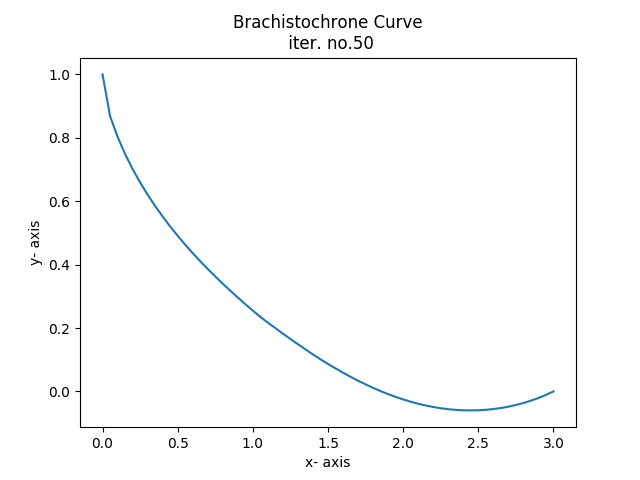
\includegraphics[width=5cm]{curve_50.png}}
    
    \medskip
    \includegraphics[width=5cm]{{curve_100.png}}\quad
    \includegraphics[width=5cm]{{curve_200.png}}\quad
    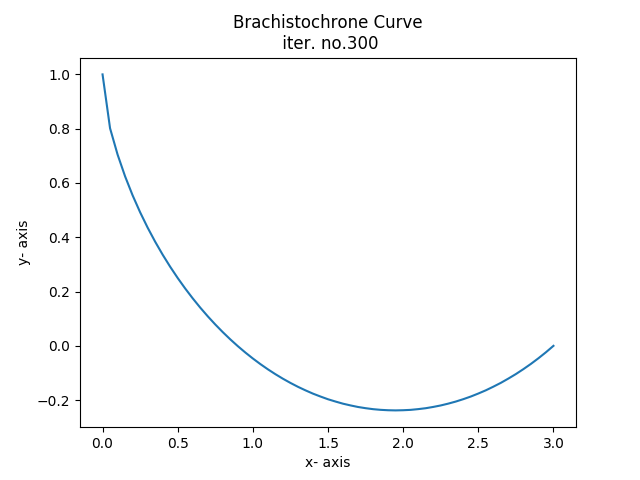
\includegraphics[width=5cm]{curve_300.png}}
    \caption{Optimization Steps and Curve Formation}
    \label{fig:curves}
\end{figure}
Here, the Brachistochrone Curve problem is treated as a optimization problem with minimizing total time taken. Laws of motion and gravity $g = 9.81 m/s^2$ is used to minimize time.\\
Equations used,
$$s = ut + \frac{1}{2}at^2$
$$v = u + at$
$$v = \frac{s}{t}$
$$a = \frac{v}{t}$

\textbf{Adam} stands for Adaptive Moment Estimation. Adam is used here as optimizer. Adam is a method that computes adaptive learning rates for each parameter.[7]\\


\begin{center}
    $*****$
\end{center}










\newpage
\section{References}
\texttt{[1] Avez, A.: Differential Calculus. J. Wiley and Sons Ltd, New York (1986)}\\
\texttt{[2] Dacorogna, B.: Introduction to the Calculus of Variations. Imperial College Press, London (2004)}\\
\texttt{[3] Markus Grasmair: Basics of Calculus of Variations}\\
\texttt{[4] Rodney Coleman: Calculus on Normed Vector Spaces (2012)} \\
\texttt{[5] Martin Burger: Infinite Dimensional Optimization and Optimal Design}\\
\texttt{[6] https://en.wikipedia.org/wiki/Brachistochrone\_curve}\\
\texttt{[7] Diederik P. Kingma, Jimmy Ba : Adam: A Method for Stochastic Optimization}\\
\texttt{[8] TensorFlow:
Large-Scale Machine Learning on Heterogeneous Distributed Systems}
\end{document}